\section{Introduction}
\label{sec:intro}

The GRTISBot X is an inexpensive, differential drive robot developed by the Georgia Robotics and Intelligent Systems Laboratory (GRITS Lab) in the Fall of 2018. It was originally designed for general multi-agent robot applications on the Robotarium \cite{robotarium,robotariumWebsite} to replace the GRITSBot \cite{GRITSBot}. The GRITSBot X is a small, versatile robot that can be deployed alone or in groups for hobby use, educational purposes, or research applications. The robot itself is almost entirely constructed of off the shelf components with a custom laser cut acrylic chassis and printed circuit board (PCB) being the only exception. The files to create these custom components (or have them fabricated externally) are found in the Github repository {\textcolor{red}{NEED CITATION WHEN MADE}}. A completed GRITSBot X can be seen in \cref{fig:GRITSBotX_Full}.

\begin{figure}[!h]
\centering
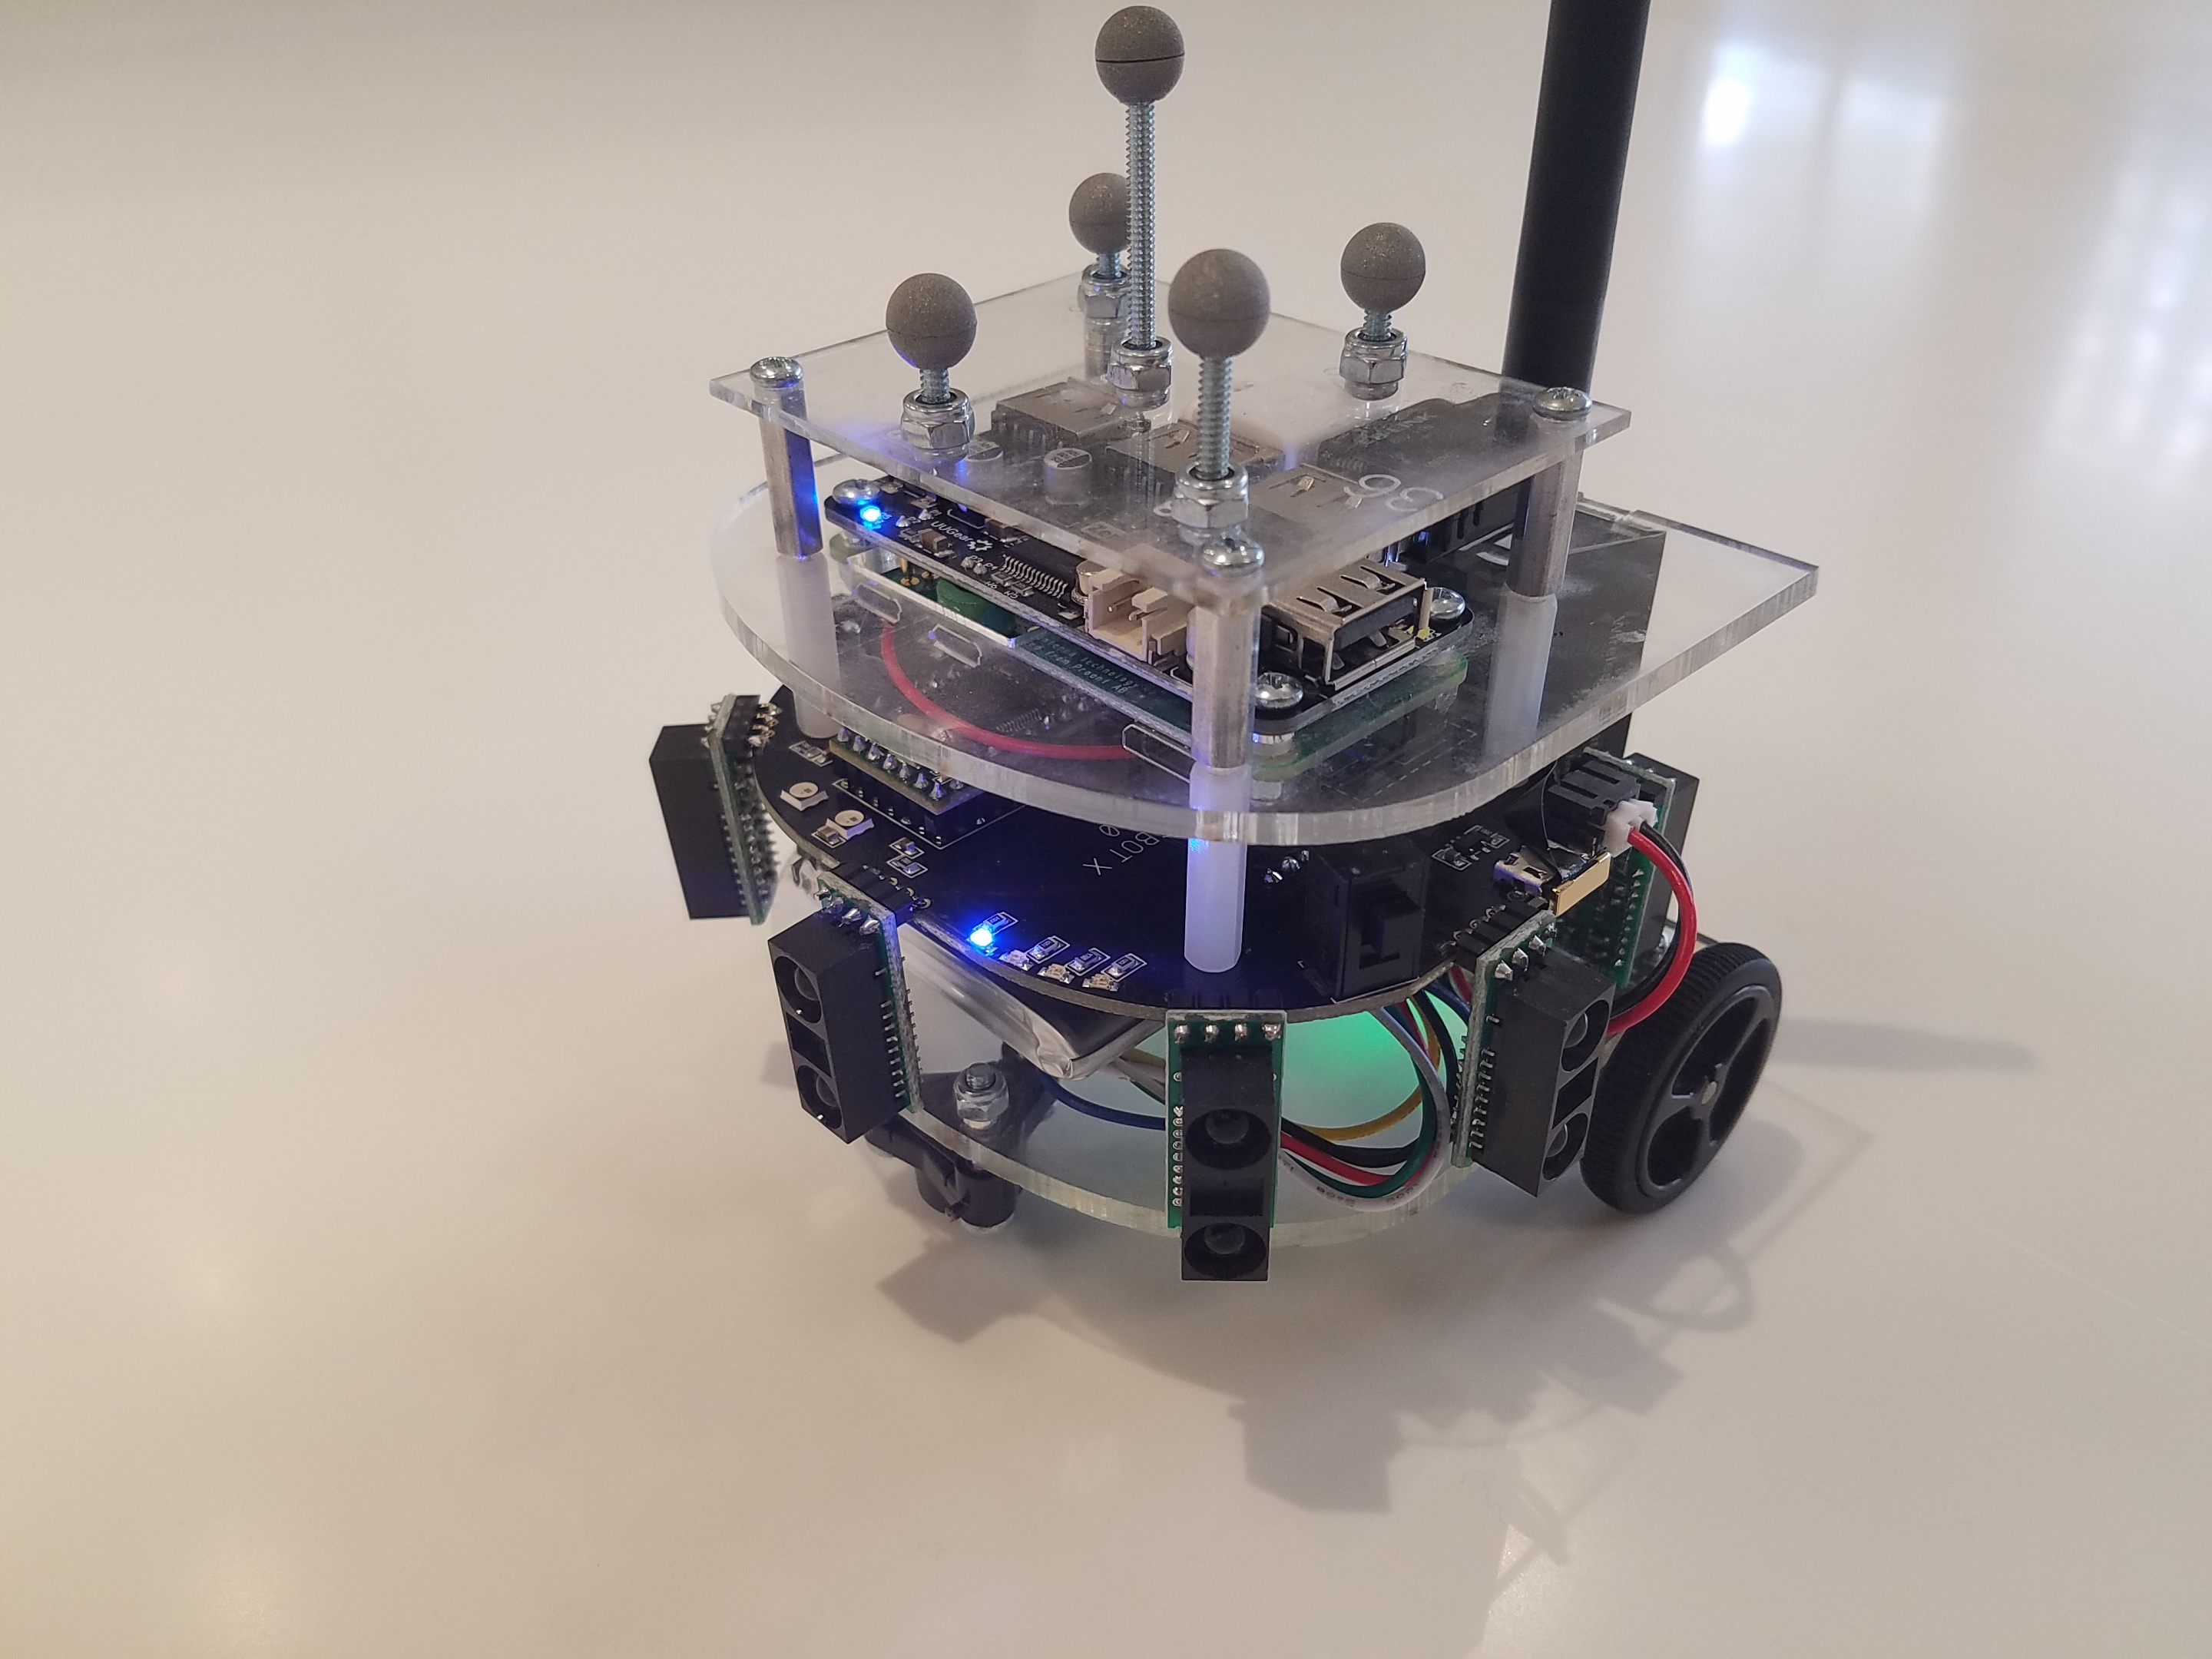
\includegraphics[width=0.65\columnwidth, keepaspectratio]{./figs/20190104_131309.jpg}
\caption{The completely assembled GRITSBot X with pearl tracking markers.}
\label{fig:GRITSBotX_Full}
\end{figure}

This document is meant as a step by step guide to construct a GRITSBot X with detailed photos and descriptions of required parts. The sections below will be broken into a short list of assembly steps with more detailed instructions on each step in the subsequent subsections. The details of each step are also linked if you are viewing the PDF on a computer. If this is your first build of the GRITSBot X, it is highly recommended that the detailed sections are read in full. The members of the GRITS Lab are glad you have chosen to take the time to build this robot. If you have any questions feel free to reach out to the contact at the top of this guide.
